\chapter{Anwendung}
\label{chap:Anwendung}

\section{Frameworks}
Die Anforderung an diese Seminararbeit war, dass Hibernate genutzt wird.
Zusätzlich habe ich mich mit Spring auseinandergesetzt. Speziell nutzte ich für diese Arbeit Spring MVC und Spring Data. Für das Logging habe ich Logback \cite{Logback} genutzt. Um die Darstellung der Web Oberfläche einfach und ansprechend zu gestalten habe ich Bootstrap \cite{Bootstrap} benutzt.

\section{Architektur}
Die Anwendung Besteht aus einer Webapplikation. Ich habe ein Model-View-Controller Ansatz gewählt wlecher mit dem Framework Spring MVC einfach umzusetzen war. Web Anfragen werden von Spring entgegengenommen und an die Controller Klassen weitergeleitet, welche die Anfrage bearbeiten.
Für das ORM habe ich Spring Data und Hibernate verwendet. 

\subsection{Dependencies}
Da es sich um ein Maven Projekt handelt werden sämtliche Dependencies über die Datei \emph{pom.xml} verwaltet.


\subsection{Struktur}
Der Source Code ist grundsätzlich in 3 Ordern untergebracht:
\begin{itemize}
	\item \emph{java}: hier sind sämtliche JAVA Klassen in verschiedenen Paketen untergebracht.
	\item \emph{resources}: hier werden Konfigurationsdateien gespeichert
	\item \emph{webapp}: hier sind die für die Web Applikation benötigten Dateien (jsp, css, js) und das web.xml gespeichert
\end{itemize}

\newpage
\subsubsection{Pakete}
Ich habe für die Anwendung den Paket Prefix ch.zhaw.schilram genutzt. Die Anwendung hat den Namen sem\_hib. Die JAVA Klassen sind in verschiedene Pakete unterteilt.
\begin{figure}[h]
\centering
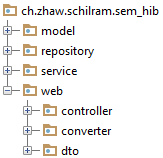
\includegraphics[width=0.2\columnwidth]{graphics/pakete.png}%
	\caption{Paketstruktur}
	\label{fig:Paketstruktur}
\end{figure}
\\
\textbf{model}\\
Im Paket \emph{model} sind die Model Klassen untergebracht welche von Hibernate für das OR Mapping genutzt werden. Sämtliche Model Klassen implementieren das Interface \emph{Uniquness}\\
\\
\textbf{repository}\\
Im Paket \emph{repository} sind sämtliche Sämtliche Interfaces welche das JPARepository Interface implementieren und für den Zugriff auf die Datenbank dienen.\\
\\
\textbf{service}\\
Das Paket \emph{service} beinhaltet für jede Model Klasse ein Service Interface und eine Service Klasse welche den Zugriff auf die Datenbank ermöglicht. Die Klasse \emph{AbstractCrudService} implementiert die CRUD Methoden welche durch die Interfaces \emph{CrudService} und \emph{ReadService} vorgegeben werden. Die Service Interfaces extenden jeweils das Interface \emph{CrudService} und werden von den Service Klassen welche auch den \emph{AbstractCrudService} extenden implementiert. Siehe dazu auch \autoref{fig:Klassendiagramm_service_repository}.  \\
\\
\textbf{web.controller}\\
Im Paket \emph{web.controller} sind die Controller Klassen abgelegt welche die Web Requests entgegennehmen und verarbeiten\\
\\
\textbf{web.converter}\\
Hier sind einerseits die Converter Klassen gespeichert, welche statische Methoden zur Umwandlung einer Model Klasse in die entsprechende DTO Klasse anbieten, sowie auch die Converter, welche gebraucht werden um über in Web Formularen als String übermittelte ID das zugehörige persistierte Objekts zu finden.\\
\\
\textbf{web.dto}\\
Im Pakte \emph{web.dto} sind die DTO bzw. Formular Klassen welche für die Formulareingabe genutzt werden abgelegt.

\subsection{Klassendiagramm}
Unten sind die Klassendiagramme der Pakete \emph{model} und \emph{service} aufgeführt.

\subsection{Klassendiagramm Paket model}

\begin{figure}[h]
\centering
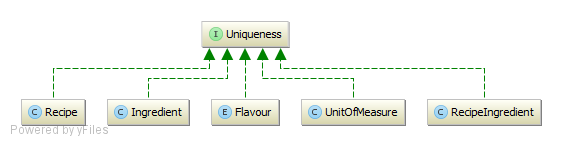
\includegraphics[width=0.6\columnwidth]{graphics/Klassendiagramm_model.png}%
	\caption{Klassendiagramm Paket \emph{model}}
	\label{fig:Klassendiagramm_model}
\end{figure}

\subsection{Klassendiagramm Pakete service und repository}
\begin{figure}[h]
\centering
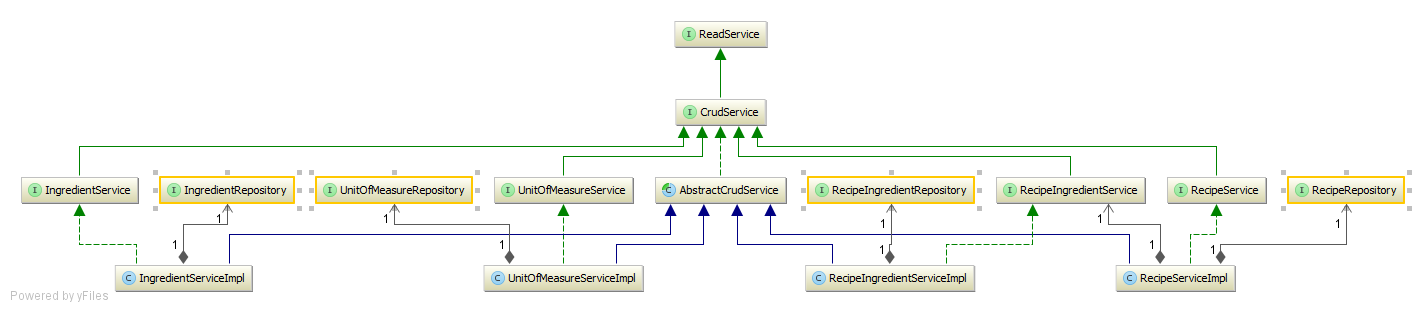
\includegraphics[width=1\columnwidth]{graphics/Klassendiagramm_service_repository.png}%
	\caption{Klassendiagramm Paket \emph{service}}
	\label{fig:Klassendiagramm_service_repository}
\end{figure}


\section{Konfigurationsfiles}\\
Im Ordner \emph{ressources} sind die Konfigurationsfiles hinterlegt.\\
\\
\textbf{application.properties}
In dieser Datei ist die Hibernate Konfiguration gespeichert. Um eine andere Datenbank oder einen anderen Datenbankuser zu verwenden müsste diese Datei angepasst werden.\\
\\
\textbf{root-context.xml}\\
Dies ist das Spring Basis Konfigurationsfile. Hier wird festgelegt in welchen Paketen Spring nach den Repository Klassen und Service Klassen sucht.\\
\\
\textbf{datasource-context.xml}\\
Hier wird Spring die Datenquelle bekanntgegeben. Die relevanten Daten werden aus dem Konfigurationsfile \emph{application.properties} ausgelesen.\\
\\
\textbf{dispatcher-context.xml}\\
Dies ist die Konfigurationsdatei für Spring MVC.\\
\\
\textbf{logback.xml}\\
Die Konfigurationsdatei für das Logging.



\section{Installation}

\subsection{Voraussetzungen}
Damit die Applikation läuft muss sie auf eine Datenbank zugreifen können. Zusätzlich wird Tomcat \cite{Tomcat} vorausgsetzt um die Web Applikation laufen zu lassen.

\subsection{Datenbank einrichten}
Die Applikation läuft mit PostgreSQL. PostgreSQL kann unter \url{http://www.postgresql.org/} heruntergeladen werden.

Nach der Installation von PostgreSQL muss der Benutzer angelegt werden. Standardmässig wird der Benutzer \emph{sem\_hib} mit dem Passwort \emph{sem\_hib} genutzt. Der Benutzer kann über das Gui oder mit folgendem SQL Statement erstellt werden.

\lstset{
	language=SQL,
	keywordstyle=\ttfamily,
	identifierstyle=\ttfamily,
	commentstyle=\color[rgb]{0.133,0.545,0.133},
	stringstyle=\ttfamily,
	showstringspaces=false,
	basicstyle=\small,
	tabsize=2,
	breaklines=true,
	prebreak = \raisebox{0ex}[0ex][0ex]{\ensuremath{\hookleftarrow}},
	breakatwhitespace=false,
	aboveskip={1.5\baselineskip},
  columns=fixed,
  upquote=true,
  extendedchars=true,
}
\begin{lstlisting}
CREATE ROLE sem_hib LOGIN
	ENCRYPTED PASSWORD 'md5198ad17e37731cbad30b3130a0a88919'
	VALID UNTIL 'infinity';
\end{lstlisting}

Nach der Erstellung des Benutzers muss noch die Datenbank erstellt werden. Der Datenbankbesitzer muss dabei auf den eben erstellten Benutzer festgelegt werden. Die Datenbank kann wahlweise über das Gui oder über das untenstehende SQL Statement erzeugt werden.

\begin{lstlisting}
CREATE DATABASE sem_hib
	WITH ENCODING='UTF8'
	OWNER=sem_hib
	CONNECTION LIMIT=-1;
\end{lstlisting}


\subsection{Tomcat einrichten}
Der Tomcat Server kann von \url{http://tomcat.apache.org/} heruntergeladen werden.
Nach der Installation von Tomcat kann die Applikation über das Management Interface installiert werden. Die Benötigte Datei heisst \emph{sem\_hib.war}. Alternativ kann dasFile \emph{sem\_hib.war} kann direkt in den Ordner \emph{webapps} von Tomcat kopiert werden.

\subsection{Applikation starten}
Nachdem die Applikation installiert ist kann über \ursl{http://localhost:8080/sem\_hib/} darauf zugegriffen werden.

\section{Applikation verwenden}
Die Applikation besteht aus den Teilen \emph{Zutaten}, \emph{Masseinheiten}, \emph{Rezepte} und \emph{Suche}.\\
Zuerst müssen Zutaten und Masseinheiten erfasst werden. Danach können diese beim Erfassen von Rezepten ausgewählt werden. Wenn einmal ein paar Rezepte erfasst sind, kann über die Suche nach Rezepten gesucht werden welche bestimmte Zutaten enthalten.

\subsection{Zutaten erfassen}
Einer Zutat kann ein Name gegeben werden und eine Beschreibung. Zusätzlich kann noch der Geschmack (Salzig, Süss, Sauer, Bitter oder Umami) agegeben werden.
\begin{figure}[h]
\centering
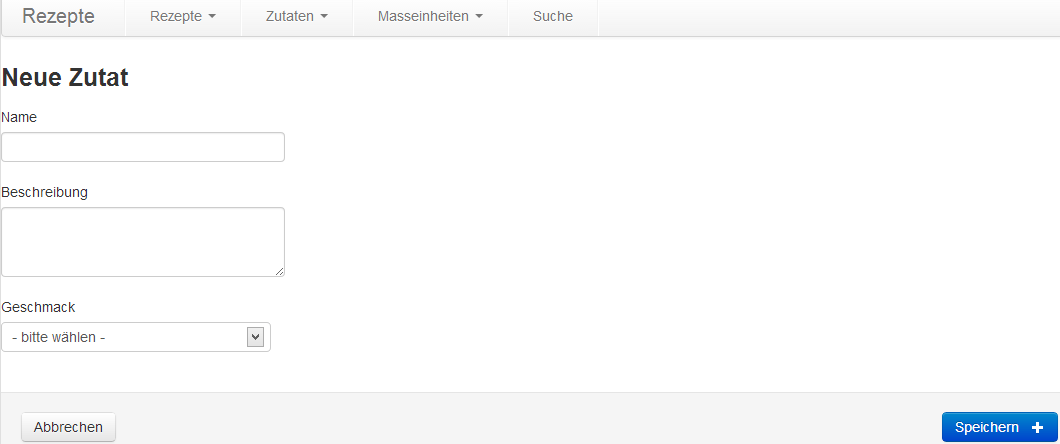
\includegraphics[width=0.5\columnwidth]{graphics/erfassen_zutat.png}%
	\caption{Zutat erfassen}
	\label{fig:erfassen_zutat}
\end{figure}

\subsection{Masseinheiten erfassen}
Der Masseinheit kann ein Key und ein Name gegeben werden. Ebenfalss kann noch eine Beschreibung hinzugefügt werden. Über den Key (z.B. EL für Esslöffel) wählt man beim Rezept dann die Masseinheit aus. 
\begin{figure}[h]
\centering
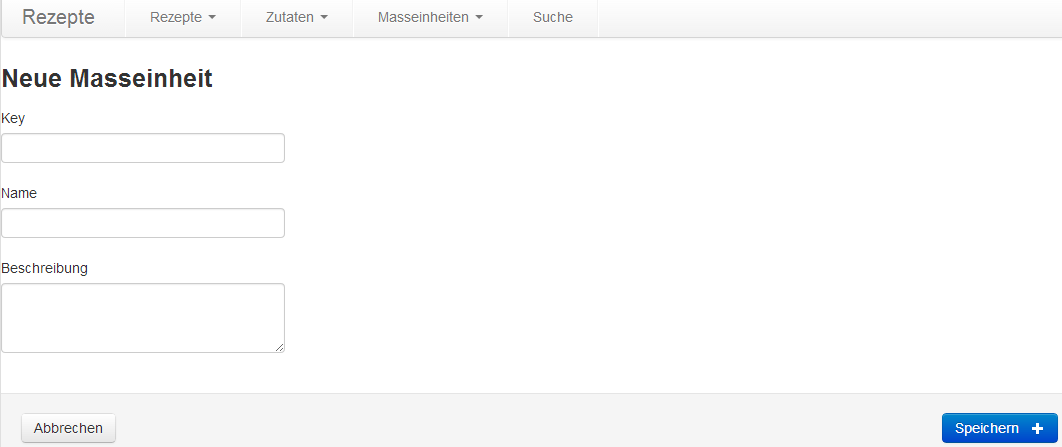
\includegraphics[width=0.5\columnwidth]{graphics/erfassen_masseinheit.png}%
	\caption{Masseinheit erfassen}
	\label{fig:erfassen_masseinheit}
\end{figure}

\subsection{Rezepte erfassen}
Beim Erfassen eines Rezeptes ist neben dem Namen natürlich wichtig, dass die Zutaten angegeben werden können. Über den Button \emph{Zeile hinzufügen} kann eine weitere Zutatenzeile hinzugefügt werden. Über das Löschen Icon neben der Zeile kann eine Zeile gelöscht werden. Im Feld \emph{Zubereitung} wird die Kochanleitung hinterlegt.
\begin{figure}[h]
\centering
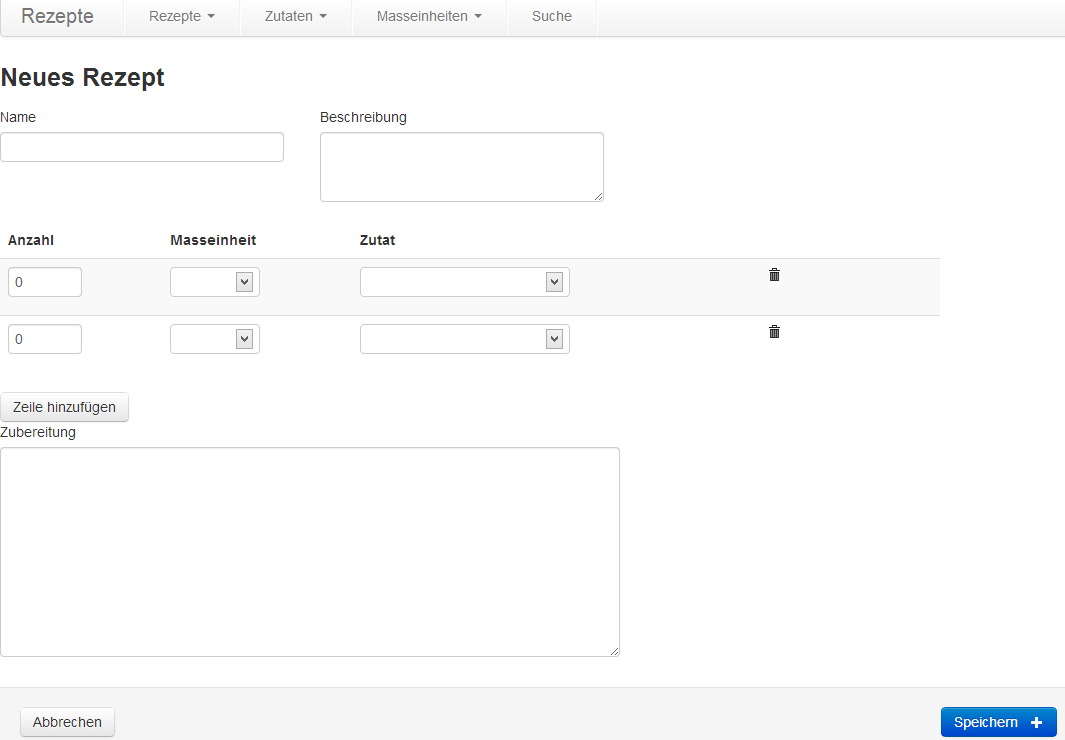
\includegraphics[width=0.5\columnwidth]{graphics/erfassen_rezept.png}%
	\caption{Rezept erfassen}
	\label{fig:erfassen_rezept}
\end{figure}

\subsection{Rezepte suchen}
Bei der Suche können bis zu drei Zutaten angegeben werden. Als Resultat werden alle Rezepte aufgelistet welche mindestens eine dieser Zutaten benötigen.